% Document Class and Basic Packages
%-------------------------------------------------------------------------------
\documentclass[letterpaper,12pt]{article} % Define the document class and options
\usepackage{graphicx} % For including graphics
\usepackage[margin=1in]{geometry}
\usepackage{cite} % Handle citations
\usepackage[final]{hyperref} % Add hyperlinks
\usepackage{pgfplotstable, booktabs} % Enhance table handling
\usepackage{placeins} % Control float placement
\usepackage{tabularray} % Advanced tables
\usepackage{titlesec} % Customize section titles
\usepackage{fancyhdr} % Create custom page headers and footers
\usepackage{empheq} % Highlight equations
\usepackage{amssymb} % Extended math symbols
\usepackage{tcolorbox} % Colored boxes
\usepackage{enumitem} % Enhanced list environments
\usepackage{xcolor} % Define custom colors
%\usepackage{parskip} % Adjust paragraph spacing
\usepackage{siunitx} % Handling SI units
\usepackage{cancel} % Strikethrough text
\usepackage{listings} % Include code listings
\usepackage{tocloft}  % Table of contents formatting
\usepackage{mathtools}
\usepackage{pdfpages}
\usepackage{times}

% 1.5 spacing equivalent to word
\usepackage{setspace}
\linespread{1.25}


% Define Custom Colors
%-------------------------------------------------------------------------------
\definecolor{codegreen}{rgb}{0,0.6,0}
\definecolor{codegray}{rgb}{0.5,0.5,0.5}
\definecolor{codepurple}{rgb}{0.58,0,0.82}

% Define Code Listing Style
%-------------------------------------------------------------------------------
\lstdefinestyle{mystyle}{
    commentstyle=\color{codegreen},
    keywordstyle=\color{codepurple},
    numberstyle=\tiny\color{codegray},
    stringstyle=\color{codegreen},
    basicstyle=\ttfamily\small,
    breakatwhitespace=false,         
    breaklines=true,                 
    captionpos=b,                    
    keepspaces=true,                                                     
    showspaces=false,                
    showstringspaces=false,
    showtabs=false,                  
    tabsize=4
}

\DeclarePairedDelimiter\abs{\lvert}{\rvert}%
\DeclarePairedDelimiter\norm{\lVert}{\rVert}%

% Swap the definition of \abs* and \norm*, so that \abs
% and \norm resizes the size of the brackets, and the 
% starred version does not.
\makeatletter
\let\oldabs\abs
\def\abs{\@ifstar{\oldabs}{\oldabs*}}
%
\let\oldnorm\norm
\def\norm{\@ifstar{\oldnorm}{\oldnorm*}}
\makeatother

% Set Code Listing Style
\lstset{style=mystyle}

% Define Custom Commands and Settings
%-------------------------------------------------------------------------------
\newcommand*\widefbox[1]{\fbox{\hspace{0em}#1\hspace{0em}}} % Create a wide box
\newcommand{\tr}{\text{tr}} % Define a trace command for math mode

% Page Header and Footer Setup
%-------------------------------------------------------------------------------
\pagestyle{fancy} % Use the fancy page style
\fancyhf{} % Clear all header and footer fields
\fancyhead[L]{MEC E 301} % Left-aligned header
\fancyhead[C]{Lab 2: Digital Measurement Techniques} % Center header
\fancyhead[R]{Alex Diep} % Right-aligned header
\fancyfoot[C]{\thepage} % Centered page number in the footer

% Section and Subsection Formatting
%-------------------------------------------------------------------------------
\titleformat*{\section}{\Large\bfseries} % Customize section titles
\titleformat*{\subsection}{\large\bfseries} % Customize subsection titles
%\renewcommand{\thesection}{Question \arabic{section}} % Modify section numbering
%\renewcommand{\thesubsection}{(\alph{subsection})} % Modify subsection numbering

% Hyperlink Setup
%-------------------------------------------------------------------------------
\hypersetup{
	colorlinks=true, % Enable colored links
	linkcolor=blue, % Set link color
	citecolor=blue, % Set citation color
	filecolor=magenta, % Set file link color
	urlcolor=blue % Set URL link color
}

% Indentation Setup
%-------------------------------------------------------------------------------
%\newcommand{\forceindent}{{\setlength{\parindent}{2em}\indent}}

% Custom SI Unit Definitions
\DeclareSIUnit\LSB{LSB} % Least significant bit

% Custom Table of Contents Formatting
\renewcommand\cftsecdotsep{\cftdot} % Use dots for section 
\renewcommand{\cftsecleader}{\cftdotfill{\cftsubsecdotsep}} % Use subsection dots for section

\sisetup{group-digits=false} % changes the default (true)
% \titlespacing\section{0pt}{12pt plus 4pt minus 2pt}{0pt plus 2pt minus 2pt}
% \titlespacing\subsection{0pt}{12pt plus 4pt minus 2pt}{0pt plus 2pt minus 2pt}
% \titlespacing\subsubsection{0pt}{12pt plus 4pt minus 2pt}{0pt plus 2pt minus 2pt}
\titlespacing*{\section}{0pt}{0.1\baselineskip}{0.2\baselineskip}
\titlespacing*{\subsection}{0pt}{0.1\baselineskip}{0.2\baselineskip}
\titlespacing*{\subsubsection}{0pt}{0.1\baselineskip}{0.2\baselineskip}

% End of Preamble
%-------------------------------------------------------------------------------

%++++++++++++++++++++++++++++++++++++++++
\begin{document}

\begin{titlepage}
    \centering
    \vspace*{2cm} % Adjust vertical spacing
    
    % Title
    \Huge {MEC E 301 \\Lab 2: Digital Measurement Techniques} \\
    \vspace{1cm} % Adjust vertical spacing
    
    % Author
    \Large by: Alex Diep \\
    \vspace{1cm} % Adjust vertical spacing

    % Date
    \Large Date: October 3, 2023 \\ % or manually specify a date
    \vspace{4cm} % Adjust vertical spacing

    % CCID and Student ID in smtaller font
    \normalsize CCID: abdiep \\
    \normalsize Student ID: 1664334 \\ 
    \normalsize Section: D21 \\
    
    \vfill % Fill vertical space
    
    % Additional content (e.g., university logo or other information)
    
\end{titlepage}
\renewcommand\arraystretch{1.5}

% Table of Contents (Hyperlinks set to locally black)
{
    \hypersetup{hidelinks}
    \tableofcontents
}
% use roman numerals for page numbers in table of contents
\pagenumbering{roman}

\newpage

% seperate page count for main matter
\pagenumbering{arabic}

\section{Notes}

fig 6 to 8 to compare manufacterer

fig 9 to 11 for simulated geometric equation

for equipment, explain why you're using the equipment
moment arm is to calculate torque and efficiency later

The sensitivity of the pressure transducer is $\qty{5}{\psi\per\volt}$.

A stroboscope was used to verify the RPM of the pump. At 1800 RPM, the stroboscope reading was 1798.

\underline{Why is the pressure of the pump outlet measured further ahead than the pressure of the pump inlet?}

The flow right out of the pump is turbulent, so the pressure head is not fully developed. Some distance away from the outlet, the flow becomes fully developed.

\underline{How does the equation for head change if the configuration is in parallel and series?}
For parallel, the head of both paths are averaged. For series, the head of both paths are added.
\begin{align*}
    H_{t, \text{parallel}} &= \frac{\Delta P_{A} + \Delta P_{B}}{2 \rho g} \\
    H_{t, \text{series}} &= \frac{\Delta P_{A} + \Delta P_{B}}{\rho g}
\end{align*}


% \section{Introduction}

\noindent The primary objective of this lab is to investigate and familiarize elements of digital measurements such as 
word length (number of bits), quantization, resolution, conversion rates, sampling, accuracy, and signal conditioning through the use of an Arduino Uno. 
These concepts are important in signal processing and digital communications and familiarity with them is important for future development.



% \section{Procedure}
% Requirements
% State the procedure followed in taking the data. The procedure should be organized 
% in the most concise, logical order; it does NOT need to be chronological. Use past 
% tense to tell the reader how you made the measurements. The reason for making each 
% measurement should also be given if necessary. e.g. "Stagnation pressure was measured 
% at 12 locations across the duct in order to determine average velocity". Include the make 
% and model number for important equipment used in the study. For MecE301 reports 
% this section is usually one or two paragraphs and one or two schematic figures. 
% Presenting, and referring to, a schematic diagram of the set-up saves words (and time) 
% and helps reader comprehension

\subsection{Equipment}
\noindent The following equipment was used to perform the experiment: Arduino Uno, MEC E 301 Shield, computer, oscilloscope, and jumper wires.

\subsection{Calibration}
\noindent For extensive details on the calibration procedure, refer to the precis provided by the MEC E 301 course
All measurements were taken from the serial monitor of the Arduino IDE. During calibration, different circuit components 
and reference voltages were used to measure the voltage output of the PCB.

First, measuring voltages with a 5V reference voltage was performed. As seen in Appendix \ref{sec:figures}, Figure \ref{fig:noaref}, the \texttt{5V} and \texttt{GND} 
pins on the Arduino Uno were connected to the \texttt{5V\_VIN} and \texttt{GND} pins on the PCB. The \texttt{A0} pin on the Arduino Uno was connected to the output pin,
\texttt{2.500V}. After uploading the sketch, ten values were recorded from the serial monitor. The \texttt{2.500V} output pin was then
swapped to \texttt{1.800V}, \texttt{1.024V}, and \texttt{0.102V} and ten values were recorded for each.

Next, measuring voltages with a 3.3V reference voltage and various circuit components was performed. As shown in Appendix \ref{sec:figures}, Figure \ref{fig:aref},
the AREF jumper on the MEC E 301 Shield was inserted, connecting the 3.3V reference voltage to the AREF pin on the Arduino Uno. First measurements of the voltages \texttt{2.500}, 
\texttt{1.800}, \texttt{1.024}, and \texttt{0.102} were performed with the 3.3V reference voltage. Then the output pins of the PCB were connected to the MEC E 301 Shield input-output 
pins to measure the various circuit components. The input-output pairs of [\texttt{D10\_I}, \texttt{D10\_O}], [\texttt{+/-10\_I}, \texttt{+/-10\_O}], and [\texttt{X10\_I}, 
\texttt{X10\_O}] measured voltages with a voltage divider, [-10, 10]V range, and amplifier respectively. Again, the voltages of \texttt{2.500}, \texttt{1.800}, \texttt{1.024}, 
and \texttt{0.102} were measured and recorded. Note, the amplifier only measured \texttt{0.102} because the other voltages were out of range.


% Next, measuring voltages with a 3.3V reference voltage was performed. The AREF jumper on the MEC E 301 Shield was inserted, connecting the
% 3.3V reference voltage to the AREF pin on the Arduino Uno. The code was modified to reflect the new reference voltage, \texttt{float voltage = sensorValue * (3.3 / 1024.0);}.
% The voltages \texttt{2.500}, \texttt{1.800}, \texttt{1.024}, and \texttt{0.102} were measured again and ten values were recorded for each.

% The next calibrations utilized different circuit components. Connecting the output pin on the PCB to the \texttt{D10\_I}, \texttt{+/-10\_I}, and \texttt{X10\_I} pins on 
% the MEC E 301 Shield allowed for the use of a voltage divider, [-10, 10]V range, and amplifier respectively. The \texttt{D10\_O}, \texttt{+/-10\_O}, and \texttt{X10\_O} 
% pins on the MEC E 301 Shield were connected to the \texttt{A0} pin on the Arduino Uno. The calibration voltages \texttt{2.500}, \texttt{1.800}, \texttt{1.024}, and \texttt{0.102}
% were measured again and ten values were recorded for each.

\subsection{Time Varying Voltage}
\noindent The \texttt{SINE\_OP} pin on the PCB was connected to the \texttt{A0} pin on the Arduino Uno as shown in Appendix \ref{sec:figures}, Figure \ref{fig:aref}
The code was modified to output a timestamp and voltage value and the baud rate was set to 115200. The serial monitor was opened and the voltage was recorded for 255 values. The values were 
copied into an Excel spreadsheet for analysis.

Lastly, measurement using an oscilloscope was performed. A schematic of the system is shown in Appendix \ref{sec:figures}, Figure \ref{fig:oscilloscope}. 
The \texttt{SINE\_OP} pin on the PCB was connected to the oscilloscope.  The \texttt{Autoset} button was pressed to automatically set the oscilloscope. Occasionally,
the \texttt{Autoset} needed to be set to a sawtooth wave to get a good reading. Lastly, the \texttt{Measure} button was pressed and the oscilloscope was set to 
measure the peak-to-peak voltage, frequency, and mean voltage.
% \forceindent The following procedure was followed as outlined in the lab precis \cite{lab2precis}. First, the Arduino Uno was 
% connected to the computer and the Arduino IDE was opened. The Arduino IDE was used to upload the \texttt{AnalogReadSerial} after 
% modifying the code \texttt{float voltage = sensorValue * (5.0 / 1024.0);} to correct the decimal-to-number conversion. 
% An additonal line was added \texttt{Serial.println(voltage, 3)} to print the voltage to the serial monitor with 3 decimal places. 

% First, measuring voltages with a 5V reference voltage was performed. The \texttt{5V} and \texttt{GND} pins on the Arduino Uno were 
% connected to the \texttt{5V\_VIN} and \texttt{GND} pins on the PCB. The \texttt{A0} pin on the Arduino Uno was connected to the output pin,
% \texttt{2.500V}. After uploading the sketch, ten values were recorded from the serial monitor. The \texttt{2.500V} output pin was then
% swapped to \texttt{1.800V}, \texttt{1.024V}, and \texttt{0.102V} and ten values were recorded for each. 

% Next, measuring voltages with a 3.3V reference voltage was performed. The AREF jumper on the MEC E 301 Shield was inserted, connecting the 
% 3.3V reference voltage to the AREF pin on the Arduino Uno. The code was modified to reflect the new reference voltage, \texttt{float voltage = sensorValue * (3.3 / 1024.0);}.
% The voltages \texttt{2.500}, \texttt{1.800}, \texttt{1.024}, and \texttt{0.102} were measured again and ten values were recorded for each.

% % next was using voltage divider to measure voltages
% Next, measuring voltages with a voltage divider was performed. The output pin on the PCB was connected to the \texttt{D10\_I} on the MEC E 301 Shield.
% The \texttt{D10\_O} pin on the MEC E 301 Shield was connected to the \texttt{A0} pin on the Arduino Uno. The code was modified to reflect the new range 
% of voltages, \texttt{float voltage = sensorValue * (33.0 / 1024.0);}. The voltages \texttt{2.500}, \texttt{1.800}, \texttt{1.024}, and \texttt{0.102} 
% were measured again and ten values were recorded for each.

% % using -10 to 10 v range
% Next, measuring voltages with a -10V to 10V range was performed. The \texttt{+/-10\_I} was connected to the PCB output pin. The \texttt{+/-10\_O} pin on the MEC E 301 Shield
% was connected to the \texttt{A0} pin on the Arduino Uno. The code was modified to reflect the new range of voltages, \texttt{float voltage = sensorValue * (20.0 / 1024.0) - 10.0;}.
% The voltages \texttt{2.500}, \texttt{1.800}, \texttt{1.024}, and \texttt{0.102} were measured again and ten values were recorded for each.

% %using amplifier
% Voltage measurements with an amplifier was performed. The \texttt{X10\_I} pin on the MEC E 301 Shield was connected to the PCB output pin. The \texttt{X10\_O} pin on the MEC E 301 Shield
% was connected to the \texttt{A0} pin on the Arduino Uno. The code was modified to reflect the new range of voltages, \texttt{float voltage = sensorValue * (0.33 / 1024.0);}.
% The voltages \texttt{2.500}, \texttt{1.800}, \texttt{1.024}, and \texttt{0.102} were measured again and ten values were recorded for each.

% % pcb time varying voltage
% Time varying voltage measurements were performed. The \texttt{SINE\_OP} pin on the PCB was connected to the \texttt{A0} pin on the Arduino Uno. The code was modified to reflect the new range of voltages, 
% \texttt{float voltage = sensorValue * (3.3 / 1024.0);}. The code was modified to ouptut a timestamp and voltage value and the baud rate was set to 115200. The serial monitor was opened and the
% voltage was recorded for 255 values.



% \section{Results and Discussion}
% Make a table summarizing the range, resolution, repeatability, accuracy 
% (determined from your experiments), and the manufacturer’s stated accuracy for 
% the five ways we configured the Arduino to measure analog voltages. (State the 
% range in V and all other values in mV). The resolution can be calculated using 
% Equation 5 of the lecture notes. The manufacturer claims that the accuracy of the 
% Uno’s A/D converter is +/– 2 least significant bits (in other words, +/– 2 times the 
% resolution if the voltage range is scaled by a reference voltage, voltage divider, 
% amplified etc). 
% Discuss the following:
% b) Discuss the trade-off between the resolution of the ADC and its range. 
% c) How does the repeatability compare to the accuracy?
% d) Is the accuracy of the Arduino improved using an external reference voltage of 3.3 
% V compared to the default 5 V reference voltage?
% e) The voltage sources used to calibrate the Uno have an accuracy of 0.05%. Is this 
% accuracy sufficient? Why or why not?
% f) Compare the accuracy you measured to the accuracy claimed by the manufacturer. 
% g) The voltage divider, voltage scaler circuit, and amplifier create additional error 
% when they are used with the Arduino. Assume they have an error of 1% of reading. 
% What error in mV do they cause when measuring a voltage at 0.102 V and at 2.500 
% V? Is it a significant source of error compared to the accuracy of the Arduino?

\subsection{Calibration of the Arduino Uno Results and Discussion}
\noindent The results can be found in \ref{sec:appendix-arduino-accuracy} in Table \ref{tab:arduino-accuracy-appendix}.
%\subsection{Calibration of the Arduino Uno Discussion}
%\subsubsection{Trade-off Between Resolution and Range}
The trade-off between resolution and range is that as the range increases, the resolution decreases. This is because the number of bits
available to represent the range is fixed. From Appendix \ref{sec:appendix-resolution}, if the range is multiplied by a factor of $k$, then the resolution is also multiplied by a factor of $k$, increasing resolution error.

%\subsubsection{Repeatability Compared to Accuracy}
Repeatability is the maximum deviation between two measurements of the same reference quantity. Accuracy is the maximum deviation between the
measured value and the true value. Repeatability is a measure of precision while accuracy is a measure of correctness.

%\subsubsection{Accuracy of Arduino Uno with 3.3V Reference Voltage}
% d) Is the accuracy of the Arduino improved using an external reference voltage of 3.3 
% V compared to the default 5 V reference voltage?

% from lab manual:
% As you probably noticed the accuracy of the default Ardiuno is not very good. This is 
% because the Arduino uses the voltage supplied over the USB cable by your computer as the 
% reference voltage for the analog-to-digital converter. The Arduino assumes this voltage is 
% 5 V but in reality, it can vary between 4.5 to 5.5 V depending on the computer. This can 
% result in large errors. To make much more accurate measurements a reference voltage can 
% be used with the Arduino’s A/D converter by suppling a known voltage to the AREF pin 
% on the Arduino. The MecE 301 shield contains a 3.300 V reference voltage (top left corner 
% of the shield) that can be supplied to the Arduino A/D converter. If a reference voltage is 
% used then the range of the A/D converter will be 0 V to 3.3 V. Thus, changing the reference 
% voltage also changes the range and resolution of the A/D. 

\noindent The accuracy for the 5V reference voltage is $\pm \qty{54.00}{\milli\volt}$ while the accuracy for the 3.3V reference voltage is $\pm \qty{17.00}{\milli\volt}$. The accuracy of the Arduino Uno is improved
using the 3.3V reference voltage. Many computers do not supply exactly 5V over the USB cable and the Arduino's A/D converter assumes the voltage is 5V. 
Supplying a known voltage to the AREF pin from the MEC E 301 Shield allows for more accurate measurements.

%\subsubsection{Accuracy of Voltage Sources}
% e) The voltage sources used to calibrate the Uno have an accuracy of 0.05%. Is this 
% accuracy sufficient? Why or why not?
\noindent From Appendix \ref{sec:appendix-voltage-source-accuracy}, if we use a conservative estimate for the accuracy of the voltage source, which occurs at 2.500V, then the accuracy is $\pm \qty{1.250}{\milli\volt}$. ANSI/ISA 51.1 states that the accuracy of the standard
can be ignored should the accuracy be one tenth of the instrument tested. % probably should cite this

Comparing this to the accuracy of the Arduino Uno, in Table \ref{tab:arduino-accuracy-appendix} the accuracy of 
the voltage source is sufficient for all reference values except the setup with the 3.3V reference voltage and 10x amplifier, which has an experimental accuracy of $\pm\qty{0.000}{\milli\volt}$.


%\subsubsection{Accuracy of Arduino Uno Compared to Manufacturer's Accuracy}
% f) Compare the accuracy you measured to the accuracy claimed by the manufacturer.
\noindent Referring to Appendix \ref{sec:appendix-arduino-accuracy}, the experimental accuracy was worse than the manufacturer's accuracy for all configurations 
except the 3.3V reference voltage with a 10x amplifier and the 3.3V reference voltage with a [-10, 10]V range.

The 5V reference voltage has an accuracy of $\pm\qty{54.00}{\milli\volt}$ while the manufacturer's accuracy is $\pm \qty{9.766}{\milli\volt}$. This may be attributed 
to the variable reference voltage supplied by the computer


%\subsubsection{Additional Error from Voltage Divider, Voltage Scaler, and Amplifier}
% g) The voltage divider, voltage scaler circuit, and amplifier create additional error 
% when they are used with the Arduino. Assume they have an error of 1% of reading. 
% What error in mV do they cause when measuring a voltage at 0.102 V and at 2.500 
% V? Is it a significant source of error compared to the accuracy of the Arduino?

\noindent The calculation is shown in Appendix \ref{sec:appendix-circuit-component-accuracy}. The error at 0.102V is $\pm \qty{1.020}{\milli\volt}$ and the error at 2.500V is $\pm \qty{25.00}{\milli\volt}$. The error at 0.102 
is not significant while the error at 2.500V is significant by ANSI/ISA 51.1.

\subsection{Time Varying Voltage Results and Discussion}
\noindent Graphs of the time varying voltage can be found in Appendix \ref{sec:figures}. Figure \ref{fig:10bit} shows the time varying voltage for the 10-bit Arduino Uno. 
Figure \ref{fig:5bit} shows the time varying voltage for the 5-bit Arduino Uno. 
% 5) Considering the calculations you made in part 4), discuss the following:
% a) How do the Arduino measurements of mean voltage, frequency, and peak-to-peak 
% voltage compare to the oscilloscope measurements?
% b) Is the precision uncertainty in the frequency measurements with the 10-bit or 5-bit 
% Arduino large? How could the measurement of frequency with the Arduino be 
% improved?
% c) Did the 10-bit or 5-bit Arduino measurement of peak-to-peak voltage have the 
% highest total uncertainty? Was the highest uncertainty caused by precision
% uncertainty or bias uncertainty? What recommendations would you make to
% improve the measurement of the peak-to-peak voltage with the Arduino?

%\subsection{Time Varying Voltage Discussion}
%\subsubsection{Arduino Measurements Compared to Oscilloscope Measurements}
From Appendix \ref{sec:appendix-time-varying-voltage-measurements}, Table \ref{tab:time-varying-voltage-mean-measurements},
the Arduino measurements of mean voltage, frequency, and peak-to-peak voltage are $\qty{1.135}{\volt}$, $\qty{47.266}{\hertz}$, and $\qty{1.217}{\volt}$ respectively.
The oscilloscope measurements are $\qty{1.17}{\volt}$, $\qty{48.54}{\hertz}$, and $\qty{1.28}{\volt}$ respectively. The Arduino measurements are close 
to the oscilloscope measurements. 

The 10 and 5 bit frequencies do not overlap with the oscilloscope frequency. The 5-bit peak to peak voltage and mean voltage overlap with the oscilloscope measurements.
The 10-bit peak to peak voltage and mean voltage do not overlap with the oscilloscope measurements.

%\subsubsection{Precision Uncertainty in Frequency Measurements}
From Appendix \ref{sec:appendix-time-varying-voltage-measurements}, Table \ref{tab:time-varying-frequency-measurements}, both the 10-bit 
and 5-bit Arduino have a precision uncertainty of about $\pm\qty{0.4}{\hertz}$, which is about 1\% of the measured frequency. 
The measurement of frequency with the Arduino can be improved by increasing the number of samples taken.

%\subsubsection{Uncertainty in Peak-to-Peak Voltage Measurements}
From Appendix \ref{sec:appendix-time-varying-voltage-measurements}, Table \ref{tab:time-varying-peak-to-peak-voltage-results}, 
the 5-bit measurement of peak-to-peak voltage had the highest total uncertainty. For the 5-bit measurements, for both the peak and troughs, 
the precision and systematic uncertainty were $\pm\qty{0.01031}{\volt}$ and $\pm\qty{0.05156}{\volt}$ respectively. The highest uncertainty is caused by 
systematic uncertainty.

%\subsubsection{Recommendations to Improve Peak-to-Peak Voltage Measurements}
From Table \ref{tab:time-varying-peak-to-peak-voltage-uncertainty-measurements}, the systematic and precision uncertainty were approximately
$\pm\qty{0.01}{\volt}$ and $\pm\qty{0.02}{\volt}$ respectively. Increasing the number of bits and increasing the linearity of the Arduino Uno would decrease the systematic uncertainty.
Increasing the sample rate would decrease the precision uncertainty since the samples can \textit{catch} the peak and troughs of the sine wave better.  
% \section{Conclusion}
\label{sec:conclusion}

\noindent The calibration section of the lab highlighted important concepts such as quantization, the trade-off between resolution and range, and the importance 
of a known reference voltage. The Arduino Uno was used to measure the voltage across different circuit components and reference voltages, and their 
impact on resolution, accuracy, and range was observed. The time varying voltage section of the lab highlighted the importance of sampling rate and 
resolution. Hands-on experience with an oscilloscope was obtained, and measurements were compared to the Arduino Uno. The Arduino Uno was able to
somewhat agree with the much more expensive oscilloscope. Increasing the sample rate and resolution of the Arduino Uno would allow for better agreement
with the oscilloscope.

% \newpage
% %\bibliographystyle{IEEEtran}
% %\bibliography{citations.bib}
% %\bibliography{}

\newpage
\appendix
\renewcommand\thefigure{\thesection.\arabic{figure}}    
\renewcommand\thetable{\thesection.\arabic{table}}
\section{Figures}
\label{sec:figures}
\subsection{Schematic of the system}
\begin{figure}[h]
    \centering
    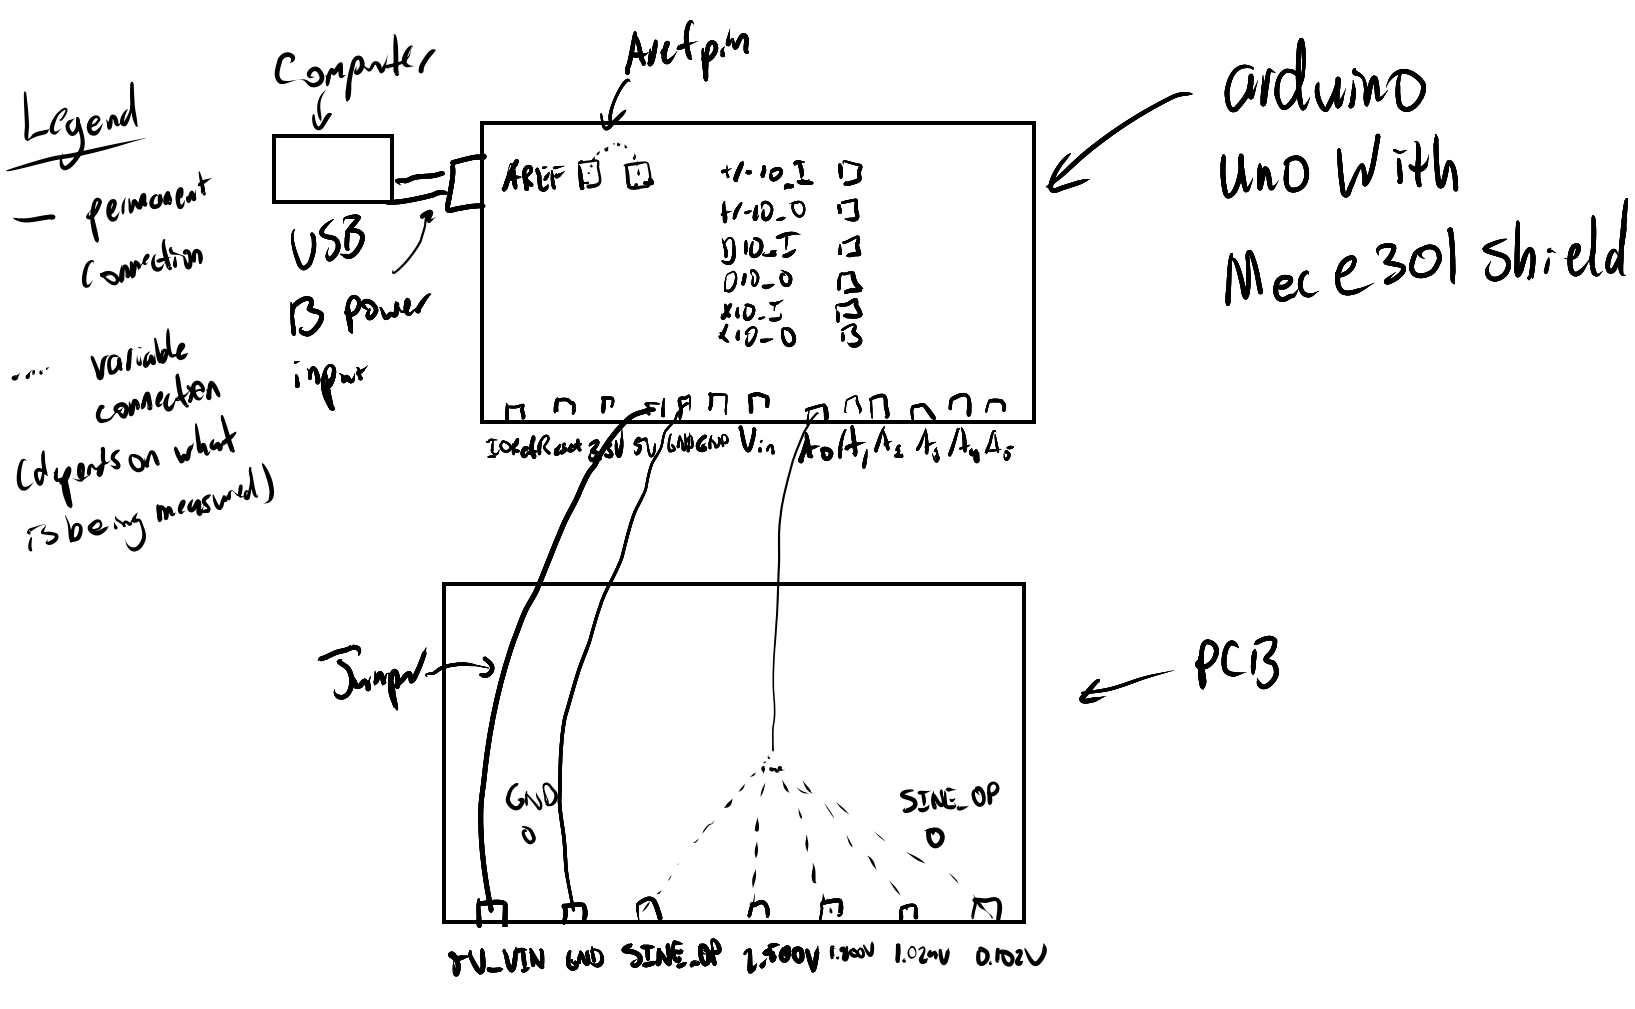
\includegraphics[width=0.5\textwidth]{Sections/Figures/noaref.png}
    \caption{Schematic of the system without a reference voltage used to measure the voltage across the PCB}
    \label{fig:noaref}
\end{figure}

\begin{figure}[h]
    \centering
    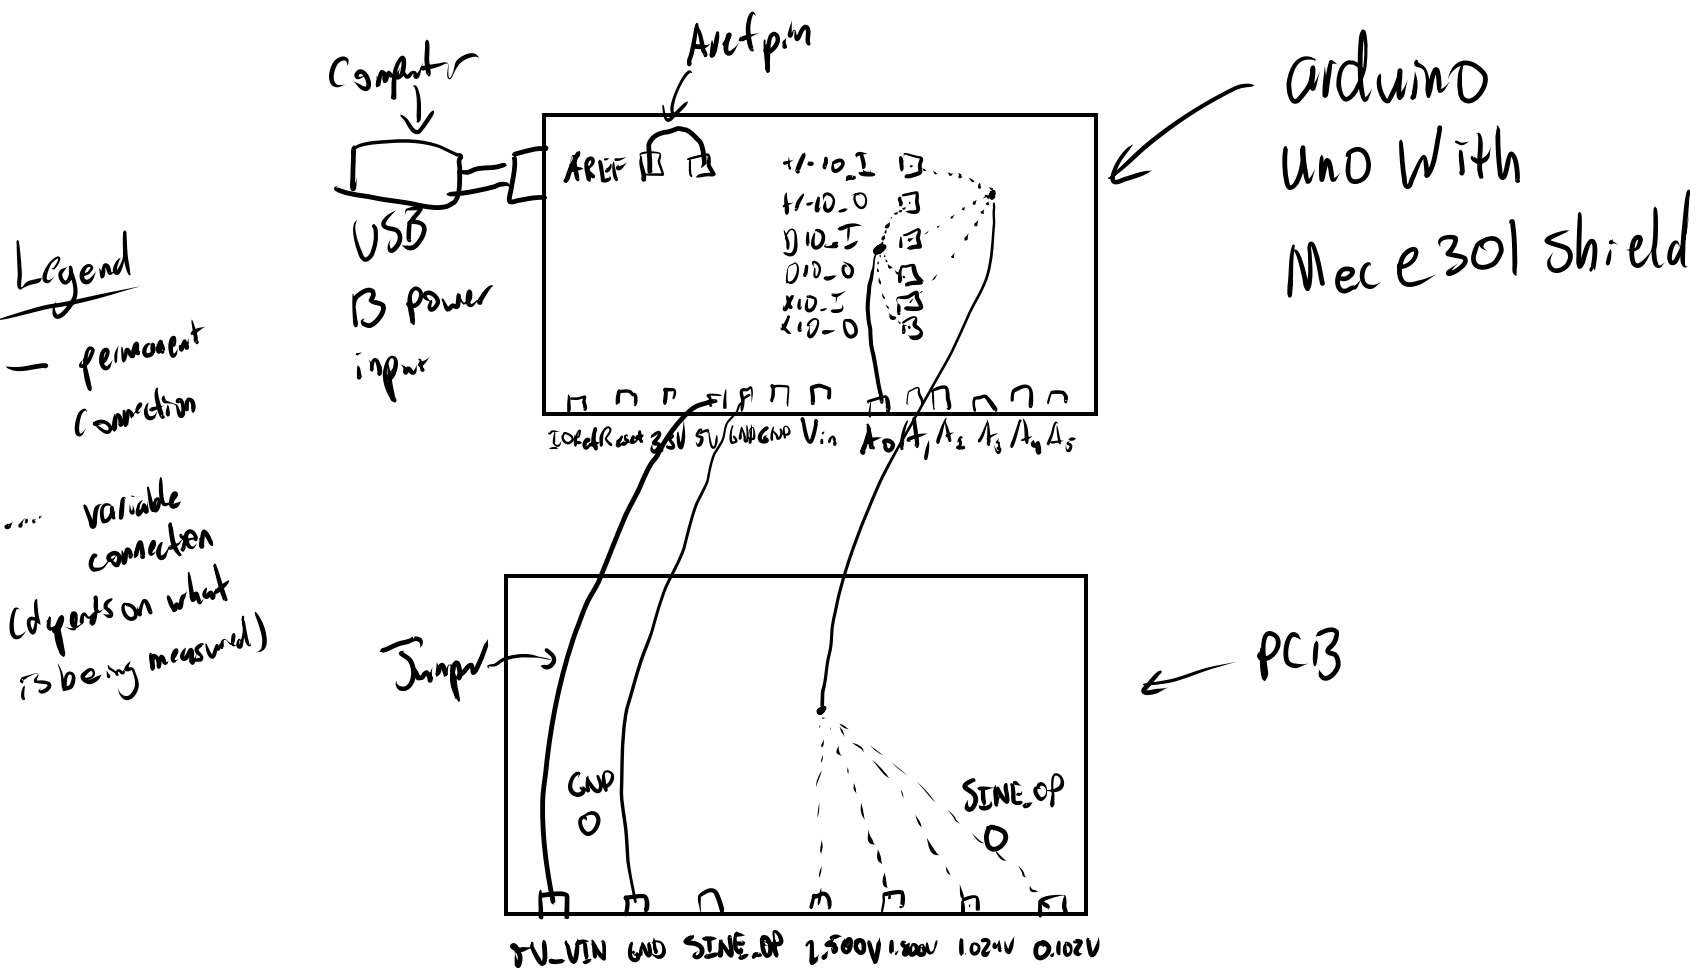
\includegraphics[width=0.5\textwidth]{Sections/Figures/aref.png}
    \caption{Schematic of the system with a 3.3V reference voltage used to measure the voltage across the PCB}
    \label{fig:aref}
\end{figure}

\begin{figure}[h]
    \centering
    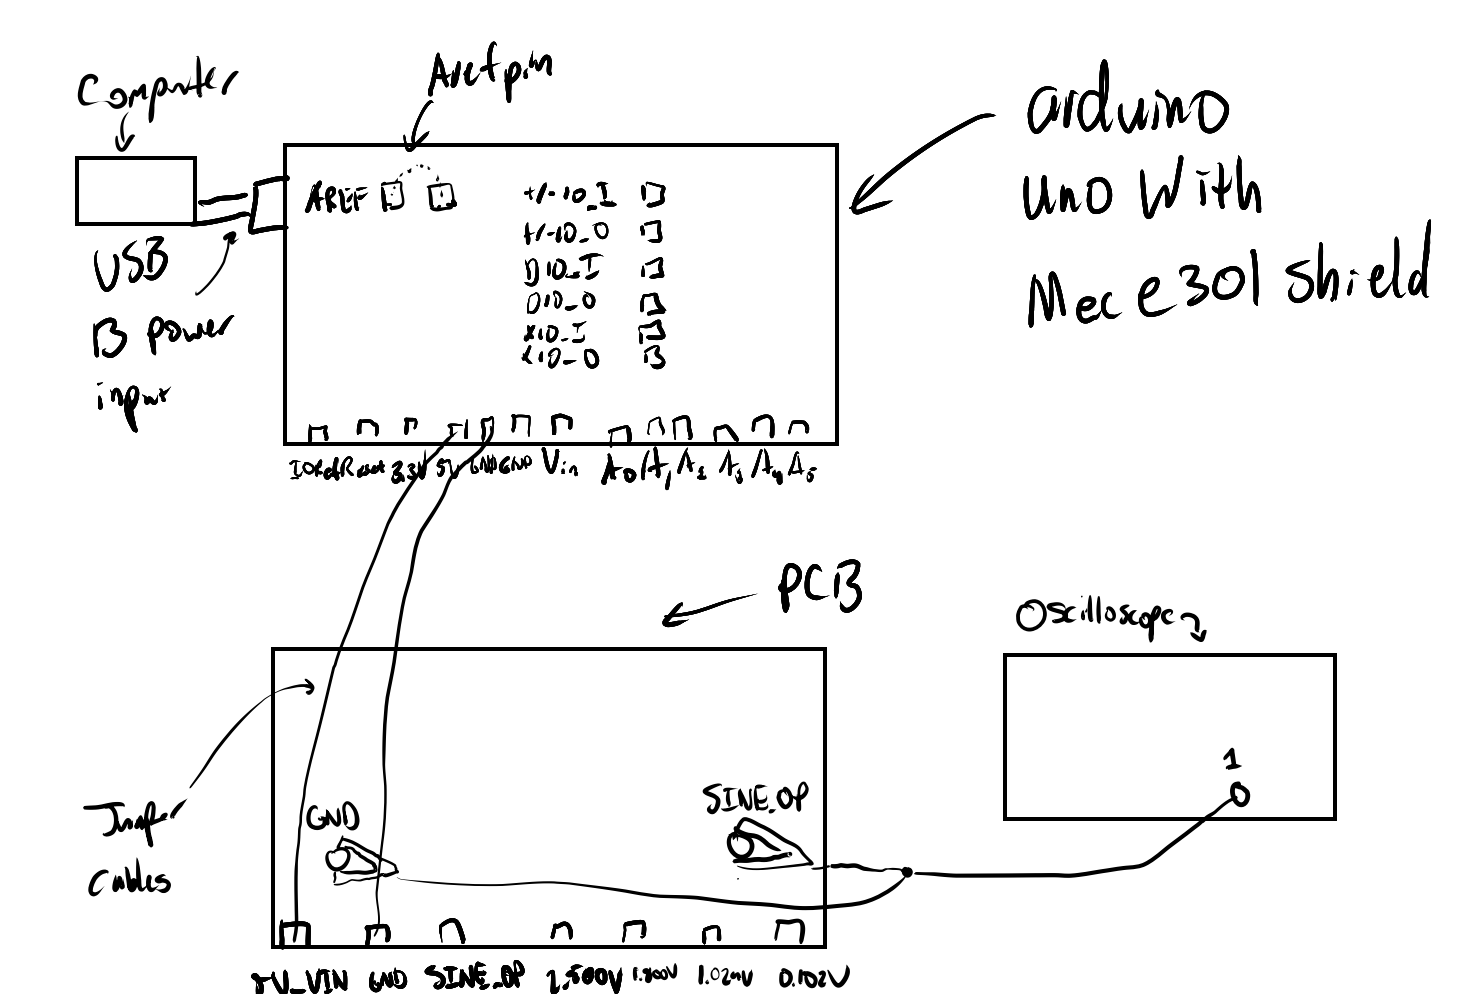
\includegraphics[width=0.5\textwidth]{Sections/Figures/oscilloscope.png}
    \caption{Schematic of the system used to measure the voltage across the PCB with an oscilloscope}
    \label{fig:oscilloscope}
\end{figure}

\FloatBarrier


\subsection{Plots of Time-Varying Signals}
\begin{figure}[h]
    \centering
    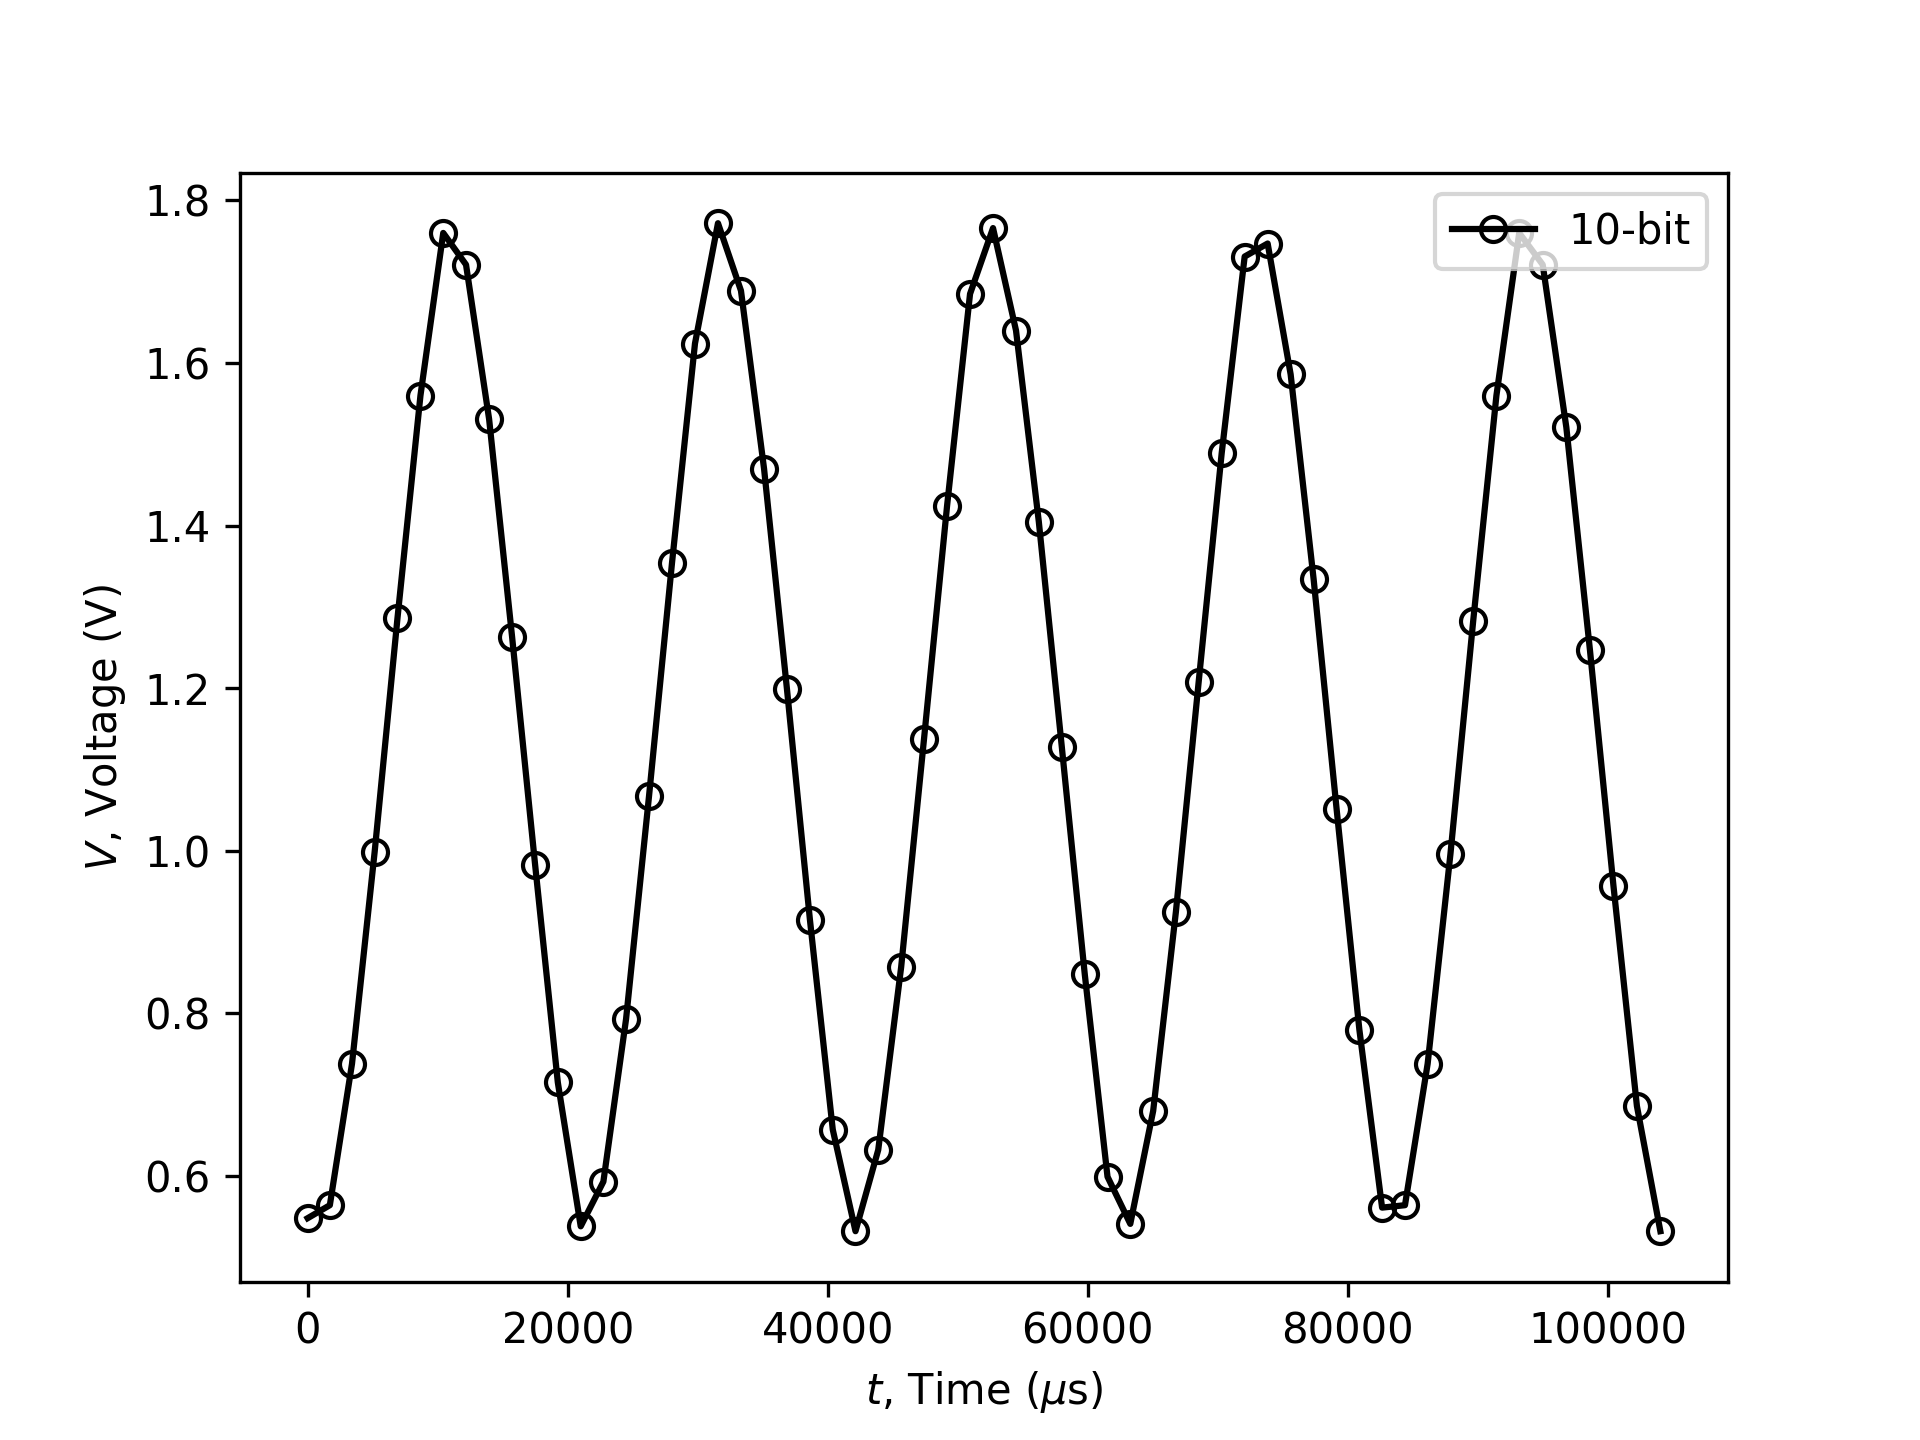
\includegraphics[width=0.5\textwidth]{Sections/Figures/10bit.png}
    \caption{Time varying signal of PCB 18 Measured with 10-bit ADC of the Arduino Uno}
    \label{fig:10bit}
\end{figure}

\begin{figure}[h]
    \centering
    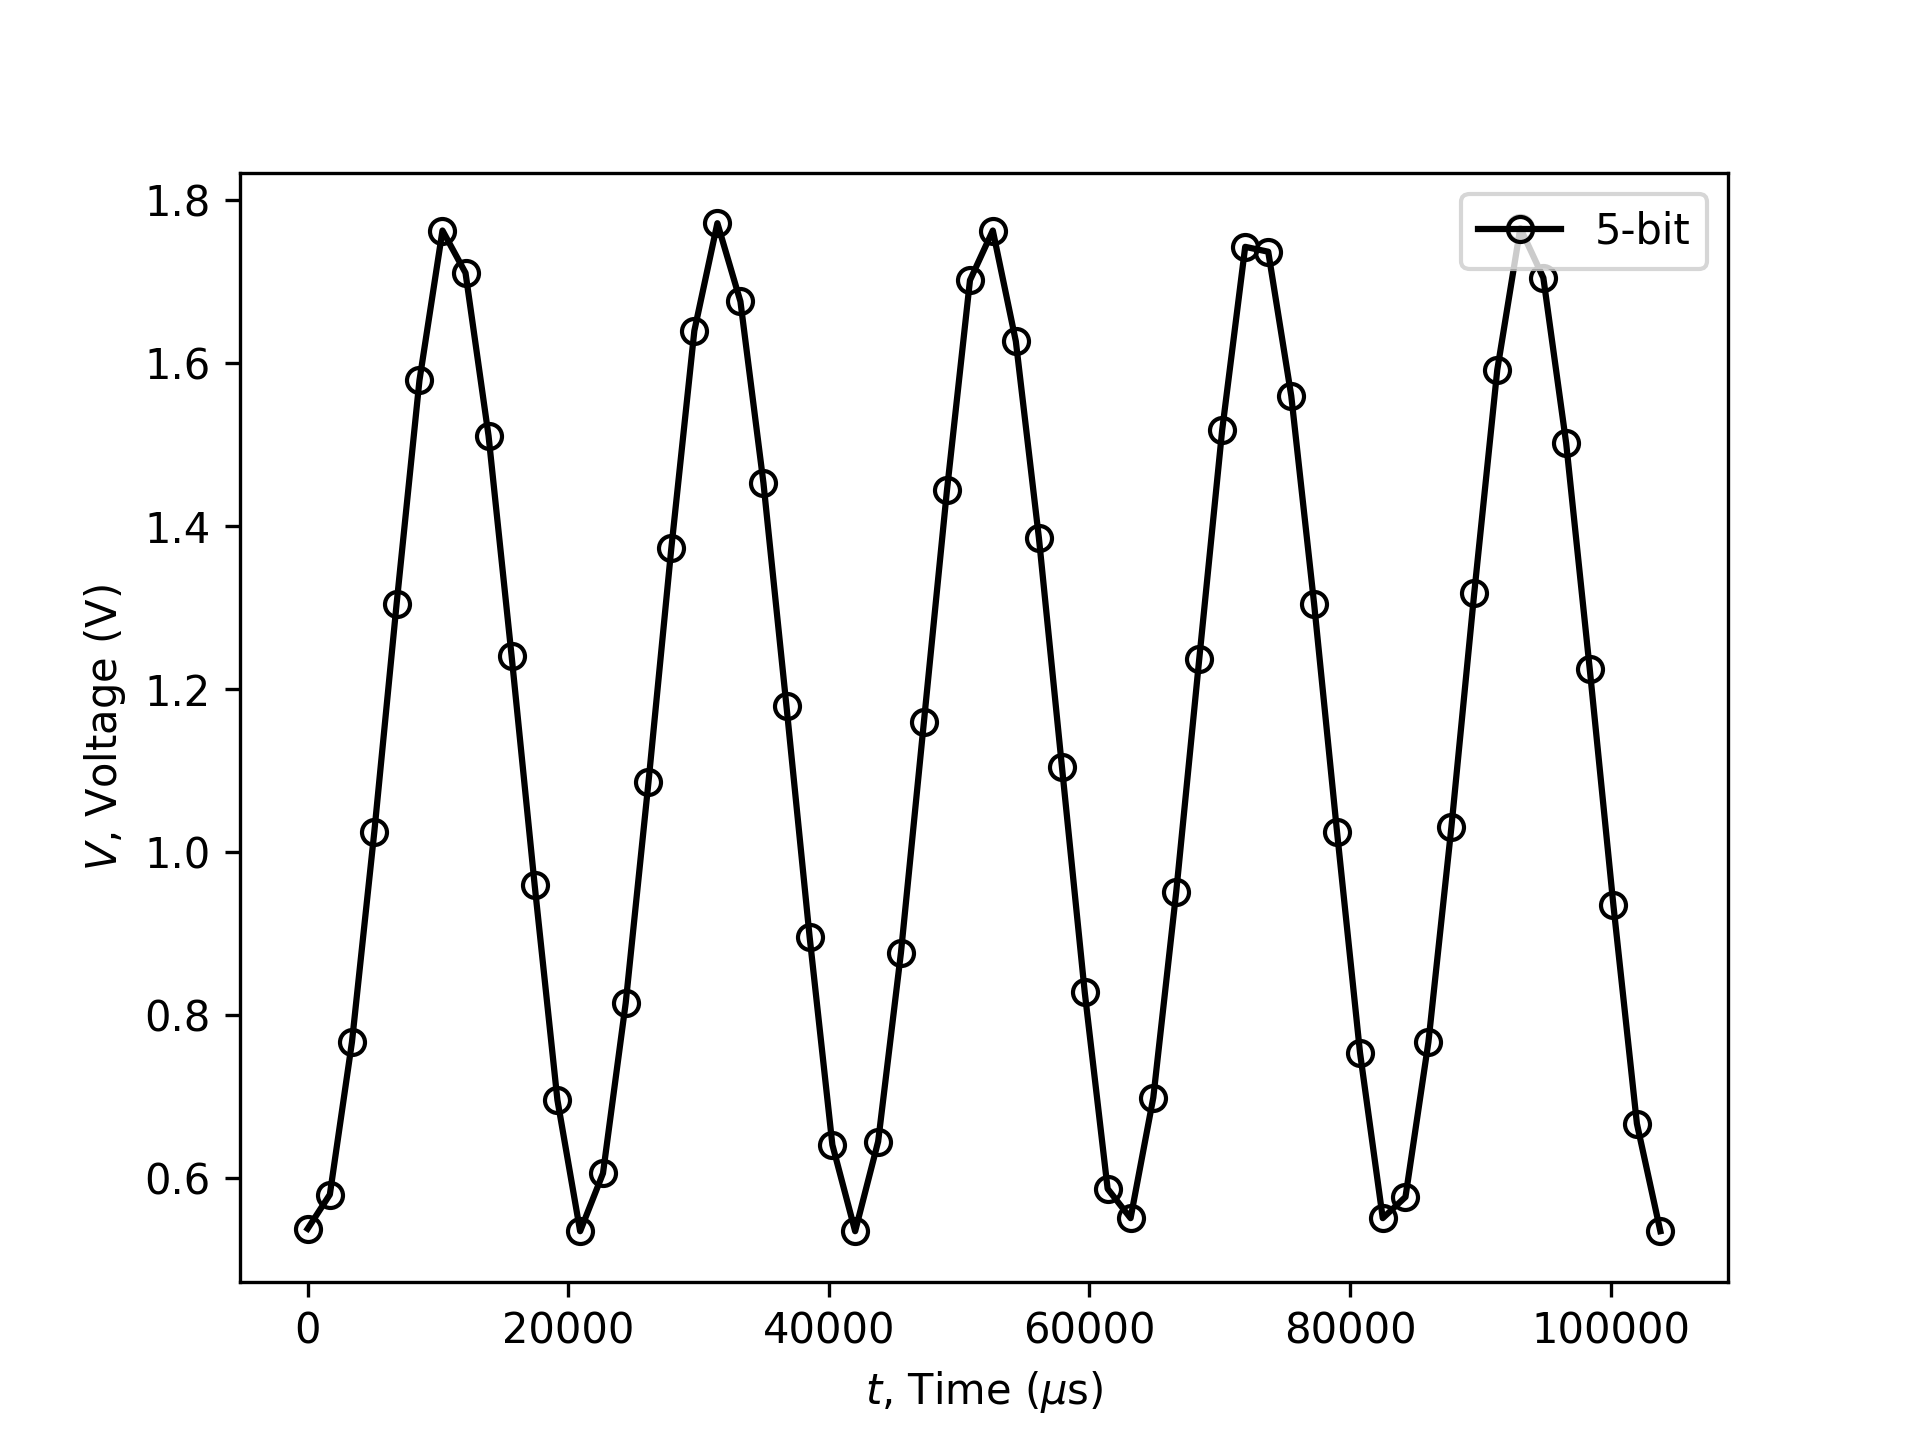
\includegraphics[width=0.5\textwidth]{Sections/Figures/5bit.png}
    \caption{Time varying signal of PCB 18 Measured with 5-bit ADC of the Arduino Uno}
    \label{fig:5bit}
\end{figure}
\FloatBarrier

% invisible character
\phantom{a}
\newpage
%\section{Appendix: Arduino Uno Calibration Results}
%\label{sec:appendix-arduino-calibration}
\begin{table}[ht]
    \caption{Range, Resolution, Repeatability, Accuracy, and Manufacturer's Accuracy for Various Ranges of the Arduino Uno}
    \label{tab:arduino-accuracy}
    \centering
    \small
    \begin{tabular}{lccccc}
        \toprule
        Arduino Config. & Range & Resolution & Repeatability & Acc. & Manuf. Acc. \\
        & (V) & (mV/LSB) & ($\pm$mV) & ($\pm$mV) & ($\pm$mV) \\
        \midrule
        5V Ref. & 0.000 - 5.000 & 4.883 & 44.00 & 54.00 & 9.766 \\
        3.3V Ref. & 0.000 - 3.300 & 3.223 & 4.000 & 17.00 & 6.445 \\
        3.3V Ref., 10x VDiv & 0.00 - 33.00 & 32.23 & 32.00 & 83.00 & 64.45 \\
        3.3V Ref., [-10, 10]V & -10.00 - 10.00 & 19.53 & 0.000 & 24.00 & 39.06 \\
        3.3V Ref., 10x Amp. & 0.000 - 0.330 & 0.3223 & 0.000 & 0.000 & 0.6445 \\
        \bottomrule
    \end{tabular}
\end{table}
%\newpage
\section{Appendix: Arduino Uno Accuracy}
\label{sec:appendix-arduino-accuracy}
Table \ref{tab:arduino-accuracy-appendix} summarizes the range, resolution, repeatability, accuracy, and manufacturer's accuracy for various ranges of the 
Arduino Uno. Sample calculations for the 5V reference voltage are shown below. Note, the manufacturer's accuracy is $\pm$ 2 LSBs.

\begin{align*}
    \text{Resolution} &= \frac{V_{\text{ru}} - V_{\text{rl}}}{2^n} \\
    &= \frac{5.000 - 0.000}{2^{10}} \\
    &= \boxed{\qty[per-mode=symbol]{4.883}{\milli\volt\per\LSB}} \\
    \text{Repeatability} &= \max({\text{Max Deviation}}) \\
    &= \max(\langle 5.00, 0.00, 9.00, 44.00 \rangle) \\
    &= \boxed{\qty{44.00}{\milli\volt}} \\
    \text{Accuracy} &= \max({\text{Deviation}}) \\
    &= \max\left(
        \tiny	
        \begin{bmatrix}
            -0.009 & -0.009 & -0.009 & -0.009 & -0.009 & -0.009 & -0.009 & -0.009 & -0.004 & -0.009 \\
            0.001 & 0.001 & 0.001 & 0.001 & 0.001 & 0.001 & 0.001 & 0.001 & 0.001 & 0.001 \\
            0.016 & 0.021 & 0.012 & 0.016 & 0.012 & 0.012 & 0.016 & 0.016 & 0.012 & 0.016 \\
            0.02 & 0.024 & 0.02 & 0.024 & 0.01 & 0.02 & \textbf{0.054} & 0.024 & 0.034 & 0.02 \\
        \end{bmatrix}
    \right) \nonumber \\
    &= \boxed{\qty{54.00}{\milli\volt}}\\
    \text{Manuf. Acc.} &= \qty{2}{\LSB} \times \text{Resolution} \\
    &= \boxed{\qty{9.766}{\milli\volt}}
\end{align*}

\noindent For significant figures, since the range is given to 3 decimal places, the resolution is given to 3 decimal places, more often
than not, the number of significant figures is 4. This is because addition and subtraction do not take into account the number of significant figures
but rather the number of decimal places.

\begin{table}[ht]
    \caption{Range, Resolution, Repeatability, Accuracy, and Manufacturer's Accuracy for Various Ranges of the Arduino Uno}
    \label{tab:arduino-accuracy-appendix}
    \centering
    \small
    \begin{tabular}{lccccc}
        \toprule
        Arduino Config. & Range & Resolution & Repeatability & Acc. & Manuf. Acc. \\
        & (V) & (mV/LSB) & (mV) & (mV) & (mV) \\
        \midrule
        5V Ref. & 0.000 - 5.000 & 4.883 & 44.00 & 54.00 & 9.766 \\
        3.3V Ref. & 0.000 - 3.300 & 3.223 & 4.000 & 17.00 & 6.445 \\
        3.3V Ref., 10x VDiv & 0.00 - 33.00 & 32.23 & 32.00 & 83.00 & 64.45 \\
        3.3V Ref., [-10, 10]V & -10.00 - 10.00 & 19.53 & 0.000 & 24.00 & 39.06 \\
        3.3V Ref., 10x Amp. & 0.000 - 0.330 & 0.3223 & 0.000 & 0.000 & 0.6445 \\
        \bottomrule
    \end{tabular}
\end{table}

\FloatBarrier
\phantom{a}
\newpage
\section{Appendix: Derivation of Resolution}
\label{sec:appendix-resolution}
\noindent The trade-off between resolution and range is that as the range increases, the resolution decreases. This is because the number of bits
available to represent the range is fixed. For example, the Arduino Uno has 10 bits to represent the range of voltages. This means that the
Arduino Uno can represent $2^{10} = 1024$ different voltages. If the range is 0 to 5V, then the resolution is 4.883mV/LSB. If the range is
0 to 10V, then the resolution is 9.766mV/LSB. 

\noindent This can be shown mathematically. Then the resolution is given by:
\[
\begin{aligned}
    \text{Resolution} &= \frac{V_{\text{ru}} - V_{\text{rl}}}{2^n} \\
\end{aligned}
\]
Let us assume the upper range $V_{\text{ru}}$ and lower range $V_{\text{rl}}$ are both multiplied by a factor of $k$.
\[
\begin{aligned}
    \text{Resolution'} &= \frac{kV_{\text{ru}} - kV_{\text{rl}}}{2^n} \\
    &= \frac{k(V_{\text{ru}} - V_{\text{rl}})}{2^n} \\
    &= k \text{Resolution} \\
\end{aligned}
\]

\
\newpage
\section{Appendix: Voltage Source Accuracy}
\label{sec:appendix-voltage-source-accuracy}

\noindent The accuracy of the voltage source is 0.05\%. A table deviation from the true value is shown below.
\begin{table}[h]
    \centering
    \caption{Deviation from True Value for Voltage Source with 0.05\% Accuracy}
    \begin{tabular}{cc}
        \toprule
        Voltage & Deviation from True Value \\
        (V) & (mV) \\
        \midrule
            0.102 & 0.051  \\
            1.024 & 0.512  \\
            1.800 & 0.900    \\
            2.500 & \textbf{1.250}  \\
        \bottomrule
    \end{tabular}
\end{table}

\noindent As one can see, the voltage source deviation is 10x smaller than the accuracy of the Arduino Uno. This means that the voltage 
source is a suitable reference voltage for the Arduino Uno.

\begin{table}[h]
    \centering
    \caption{Accuracy of Voltage Source Compared to Arduino Uno}\
    \label{tab:voltage-source-accuracy}
    \begin{tabular}{lc}
        \toprule
        Configuration & Accuracy  \\
                          & (mV)      \\
        \midrule
    Voltage Source        & 1.250      \\
    5V Ref.~              & 54.00     \\
    3.3V Ref.~            & 17.00     \\
    3.3V Ref., 10x VD     & 83.00     \\
    3.3V Ref., [-10, 10]V & 24.00     \\
    3.3V Ref., 10x Amp.~  & 0.000    \\
    \bottomrule
    \end{tabular}
\end{table}
\newpage
\section{Appendix: Circuit Component Accuracy}
\label{sec:appendix-circuit-component-accuracy}
Below is a table of the additional error from the voltage divider, voltage scaler, and amplifier. The error is calculated by multiplying the voltage by 1\%.

\begin{table}[h]
    \centering
    \caption{Additional Error from Voltage Divider, Voltage Scaler, and Amplifier}
    \begin{tabular}{cc}
        \toprule 
        Voltage & Error \\
        (V) & ($\pm$mV) \\
        \midrule
    0.102 & 1.020  \\
    2.500 & 25.00 \\
    \bottomrule
    \end{tabular}
\end{table}
\newpage
\section{Time-Varying Voltage Measurements}
\label{sec:appendix-time-varying-voltage-measurements}

\noindent Below in Table \ref{tab:time-varying-voltage-mean-measurements} are the nominal measurements for the time-varying voltage for the 10-bit and 5-bit ADCs.
\begin{table}[h]
    \centering
    \caption{Nominal Measurements of Time-Varying Voltage}
    \label{tab:time-varying-voltage-mean-measurements}
    \begin{tabular}{lccc}
      \toprule
           & \multicolumn{3}{c}{Mean Measurements of Time-Varying Voltage} \\
    \cmidrule{2-4}
           & Frequency & Peak to Peak & Mean Voltage       \\
           & (Hz)      & (V)          & (V)           \\
    \midrule
    10-bit & 47.266  & 1.217        & 1.135         \\
    5-bit  & 47.372  & 1.2194       & 1.144         \\
    Oscilloscope & 48.54 & 1.28 & 1.17 \\
   \bottomrule
    \end{tabular}
\end{table}
\subsection{Mean Sample Calculation}
\noindent The mean voltage for the 10-bit and 5-bit ADCs was calculated using Excel using the \texttt{=AVERAGE()} function across 5 cycles, which was
approximately 60 data points. 

\subsection{Time-Varying Voltage Period Measurements}

\noindent Below is a table of the time-varying period measurements for the 10-bit and 5-bit ADCs. 
\begin{table}[h]
    \centering
    \caption{Time-Varying Period Measurements for 10-bit and 5-bit ADCs}
    \begin{tabular}{lcccccc}
    \toprule
       & \multicolumn{5}{c}{Period ($\mu$s)}    \\
    \cmidrule{2-6}
       & Cycle 1    & Cycle 2   & Cycle 3   & Cycle 4   & Cycle 5    \\
    \midrule
    10-bit & 21000 & 21132 & 21132 & 21124 & 21400  \\
    5-bit  & 20912 & 21104 & 21136 & 21096 & 21304  \\
    \bottomrule
    \end{tabular}
\end{table}

\noindent \textbf{Obtaining the nominal value (mean)}, standard deviation, and T-distribution inverse was done through Excel. The mean was calculated using the \texttt{=AVERAGE()} function 
across 5 cycles, which was approximately 60 data points. The standard deviation was calculated using the \texttt{=STDEV.S()} function. 
The T-distribution inverse was calculated using the \texttt{=T.INV()} function, where $\alpha = 0.05$ and $n = 5$. The results are shown in Table 
\ref{tab:time-varying-period-uncertainty-measurements}.

\begin{table}[h]
   \centering
   \caption{Time-Varying Period Uncertainty Measurements for 10-bit and 5-bit ADCs}
   \label{tab:time-varying-period-uncertainty-measurements}
   \begin{tabular}{lcccccc}
      \toprule
      & Nominal Value & STDEV & T-Inv & $P_x$ \\
      & ($\mu$s)      & ($\mu$s)           &                        & ($\pm\mu$s)    \\
      \midrule
      10-bit & 21158 & 146.66 & 2.7764 & 182.10 \\
      5-bit  & 21110 & 139.42 & 2.7764 & 173.11 \\
      \bottomrule
   \end{tabular}
\end{table}

Sample calculations for the \textbf{10-bit} ADC are shown. To calculate the random uncertainty, the following equation was used:
\[
\begin{aligned}
   P_x &= t_{\alpha/2, n-1} \frac{\sigma}{\sqrt{n}} \\
         &= 2.7764 \frac{\qty{146.66}{\micro\second}}{\sqrt{5}} \\
         &= \boxed{\qty{182.10}{\micro\second}}
\end{aligned}
\]

\subsection{Time-Varying Voltage Frequency Calculations}
%\noindent Below is a table of the time-varying frequency measurements for the 10-bit and 5-bit ADCs.
% Frequency	
% nominal value	Uncertainty
% 10-Bit	47.264	0.40680
% 5-Bit	47.370	0.38844
\begin{table}[h]
   \centering
   \caption{Time-Varying Frequency Results for 10-bit and 5-bit ADCs}
   \label{tab:time-varying-frequency-measurements}
   \begin{tabular}{lcc}
   \toprule
      & \multicolumn{2}{c}{Frequency}    \\
      & (Hz) & ($\pm$Hz) \\
   \cmidrule{2-3}
   & Nominal Value & Uncertainty \\
   \midrule
   10-bit & 47.264 & 0.40680 \\
   5-bit  & 47.370 & 0.38844 \\
   \bottomrule
   \end{tabular}
\end{table}

\noindent The equation relating frequency and period is shown below. Sample calculation for the 10-bit ADC is shown below.
\[
\begin{aligned}
   f &= \frac{1}{T} \\
       &= \frac{1}{\qty{21158}{\micro\second}} \\
       &= \boxed{\qty{47.264}{\hertz}}
\end{aligned}
\]

\noindent Utilizing error propagation, the random uncertainty in frequency is:
\[
\begin{aligned}
   P_{x'} &= \sqrt{\left(\frac{\partial f}{\partial T} P_x\right)^2} \\
         &= \abs{\frac{\partial f}{\partial T} P_x} \\
         &= \abs{-\frac{1}{T^2} P_x} \\
         &= \frac{P_x}{T^2}\\
         &= \frac{\qty{182.10}{\micro\second}}{\qty{21158}{\micro\second}^2}\\
         &= \boxed{\qty{0.40680}{\hertz}}
\end{aligned}
\]

\subsection{Time-Varying Voltage Peak to Peak Voltage Calculations}
\noindent Below are the resulting peaks and troughs for the 10-bit and 5-bit ADCs for 5 cycles. 
\begin{table}
   \centering
   \caption{Time-Varying Peak and Trough Voltage Measurements for 10-bit and 5-bit ADCs}
   \label{tab:time-varying-peak-to-peak-voltage-measurements} 
   \begin{tabular}{lcccccc}
   \toprule
      & \multicolumn{5}{c}{Peak and Trough Voltage (V)}    \\
   \cmidrule{2-6}
      & Cycle 1    & Cycle 2   & Cycle 3   & Cycle 4   & Cycle 5    \\
   \midrule
   10-bit Trough & 1.212 & 1.234 & 1.234 & 1.206 & 1.199  \\
   5-bit Trough  & 1.225 & 1.237 & 1.228 & 1.192 & 1.215  \\
   10-bit Peak   & 1.763 & 1.772 & 1.763 & 1.743 & 1.766  \\
   5-bit Peak    & 1.76  & 1.772 & 1.766 & 1.747 & 1.76   \\
   \bottomrule
   \end{tabular}
\end{table}


\noindent \textbf{The nominal values for troughs and peaks} were calculated using the \texttt{=AVERAGE()} function in Excel, the standard deviation 
was calculated using the \texttt{=STDEV.S()} function, and the T-distribution inverse was calculated using the \texttt{=T.INV()} function, where $\alpha = 0.05$ 
and $n = 5$. The systematic uncertainty was taken to be the accuracy of the 3.3V reference voltage for 10-bit ADC. and half the resolution for 5-bit ADC.

\begin{table}[h]
   \centering
   \caption{Time-Varying Peak and Trough Voltage Uncertainty Measurements for 10-bit and 5-bit ADCs}
   \label{tab:time-varying-peak-to-peak-voltage-uncertainty-measurements}
   \begin{tabular}{lcccccc}
      \toprule
      & Nominal Value & STDEV & T-Inv & $P_x$ & $B_x$ & $U_x$ \\
      & (V)           & (V)                &       & ($\pm$V)   & ($\pm$V)   & ($\pm$V)   \\
      \midrule
      10-bit Trough & 0.544 & 0.01111 & 2.7764 & 0.01380 & 0.01700 & 0.0219 \\
      5-bit Trough  & 0.542 & 0.008307 & 2.7764 & 0.01031 & 0.05156 & 0.0526 \\
      10-bit Peak   & 1.761 & 0.009274 & 2.7764 & 0.01151 & 0.01700 & 0.0205 \\
      5-bit Peak    & 1.761 & 0.01092 & 2.7764 & 0.01356 & 0.05156 & 0.0533 \\
      \bottomrule
   \end{tabular}
\end{table}
\FloatBarrier
\noindent The total uncertainty, $U_x$, was calculated using the root sum square (RSS) method. An example calculation for the 10-bit trough is shown below:
\[
   \begin{aligned}
      U_x &= \sqrt{P_x^2 + B_x^2} \\
            &= \sqrt{0.01380^2 + 0.01700^2} \\
            &= \boxed{\qty{0.0219}{\volt}}
   \end{aligned}
\]

\noindent Obtaining peak to peak voltage was done by subtracting the trough from the peak. The results are shown in Table \ref{tab:time-varying-peak-to-peak-voltage-results}. 
A sample calculation for 10-bit ADC and equation for peak to peak voltage is shown below:
\[
\begin{aligned}
   V_{\text{p-p}} &= V_{\text{ru}} - V_{\text{rl}} \\
                  &= \qty{1.761}{\volt} - \qty{0.544}{\volt} \\
                  &= \boxed{\qty{1.217}{\volt}}
\end{aligned}
\]

\begin{table}[h]
   \centering
   \caption{Time-Varying Peak to Peak Voltage Results for 10-bit and 5-bit ADCs}
   \label{tab:time-varying-peak-to-peak-voltage-results}
   \begin{tabular}{lcc}
   \toprule
   & Nominal Value & $U_x$ \\
   & (V)           & ($\pm$V)   \\
   \midrule
   10-bit & 1.217 & 0.0381  \\
   5-bit  & 1.219 & 0.0981   \\
   \bottomrule
   \end{tabular}
\end{table}
\FloatBarrier
\noindent Error propagation was used to calculate the uncertainty in peak to peak voltage. The equation for peak to peak voltage is shown below with 
sample calculations for the 10-bit ADC.
\[
\begin{aligned}
   U_{x'} &= \sqrt{\left(\frac{\partial V_{\text{p-p}}}{\partial V_{\text{ru}}} U_{x, ru}\right)^2 + \left(\frac{\partial V_{\text{p-p}}}{\partial V_{\text{rl}}} U_{x, rl}\right)^2} \\
          &= \sqrt{1^2 0.0219^2 + (-1)^2 0.0205^2} \\
            &= \boxed{\qty{0.0381}{\volt}}
\end{aligned}
\]



% \begin{table}[h]
%     \centering
%     \caption{Time-Varying Frequency Measurements for 10-bit and 5-bit ADCs}
%     \begin{tabular}{lcccccc}
%     \toprule
%        & \multicolumn{5}{c}{Frequency (Hz)}    \\
%     \cmidrule{2-6}
%        & Cycle 1    & Cycle 2   & Cycle 3   & Cycle 4   & Cycle 5    \\
%     \midrule
%     10-bit & 47.619 & 47.295 & 47.331 & 47.357 & 46.729  \\
%     5-bit  & 47.819 & 47.384 & 47.313 & 47.402 & 46.940  \\
%     \bottomrule
%     \end{tabular}
% \end{table}

% \begin{table}[h]
%     \centering
%     \caption{Time-Varying Peak to Peak Voltage Measurements for 10-bit and 5-bit ADCs}
%     \begin{tabular}{lcccccc}
%     \toprule
%        & \multicolumn{5}{c}{Peak to Peak Voltage (V)}    \\
%     \cmidrule{2-6}
%        & Cycle 1    & Cycle 2   & Cycle 3   & Cycle 4   & Cycle 5    \\
%     \midrule
%     10-bit & 1.212 & 1.234 & 1.234 & 1.206 & 1.199  \\
%     5-bit  & 1.225 & 1.237 & 1.228 & 1.192 & 1.215  \\
%     \bottomrule
%     \end{tabular}
% \end{table}

% \begin{table}[h]
%     \centering
%     \label{tab:time-varying-voltage-mean-measurements}
%     \begin{tabular}{lccc}
%            & \multicolumn{3}{c}{Mean Measurements of Time-Varying Voltage} \\
%     \cmidrule{2-4}
%            & Frequency & Peak to Peak & Voltage       \\
%            & (Hz)      & (V)          & (V)           \\
%     \midrule
%     10-bit & 47.266  & 1.217        & 1.135         \\
%     5-bit  & 47.372  & 1.2194       & 1.144         \\
%     Oscilloscope & 48.54 & 1.28 & 1.17 \\
%    \bottomrule
%     \end{tabular}
% \end{table}
% \subsection{Mean Sample Calculation}
% The mean for the 10-bit and 5-bit ADCs was calculated using Excel using the \texttt{=AVERAGE()} function across 5 cycles, which was
% approximately 60 data points. 

% \subsection{Uncertainty Analysis}
% \subsubsection{Frequency Uncertainty}
% \noindent Sample calculations for the 10-bit ADC are shown below. Note that the 5-bit ADC calculations are similar.

% For frequency, standard deviation, $\sigma$, was calculated from Excel using \texttt{=STDEV.S()}.
% For the T-distribution inverse, $t_{\alpha/2, n-1}$, the \texttt{=T.INV()} function was used, where
% $\alpha = 0.05$ and $n = 5$.

% \noindent Using $\sigma = \qty{0.32582}{\hertz}$ and $t_{\alpha/2, n-1} = 2.7764$, the uncertainty in frequency is:
% \[
% \begin{aligned}
%       u(f) &= t_{\alpha/2, n-1} \frac{\sigma}{\sqrt{n}} \\
%             &= 2.7764 \frac{\qty{0.32582}{\hertz}}{\sqrt{5}} \\
%             &= \qty{0.40456}{\hertz}
% \end{aligned}   
% \]

% \subsubsection{Peak to Peak Voltage Uncertainty}
% \noindent For peak to peak voltage, $\sigma = 0.0162$ and $t_{\alpha/2, n-1} = 2.7764$, so the uncertainty in peak to peak voltage is:
% \[
% \begin{aligned}
%       P_x &= t_{\alpha/2, n-1} \frac{\sigma}{\sqrt{n}} \\
%                 &= 2.7764 \frac{\qty{0.0162}{\volt}}{\sqrt{5}} \\
%                   &= \qty{0.0201}{\volt}
% \end{aligned}
% \]

% \noindent For $B_x$, error propagation was used. For a single measurement, the systematic uncertainty was
% $B_{x} = \qty{0.01700}{\volt}$, which was taken from the calibration of the 3.3V reference section. 
% Since the governing equation is:
% \[
% \begin{aligned}
%       V_{\text{p-p}} &= V_{\text{ru}} - V_{\text{rl}}
% \end{aligned}
% \]
% \noindent The propagated systematic uncertainty is:
% \[
%    \begin{aligned}
%       B_{x'} &= \sqrt{\frac{\partial V_{\text{p-p}}}{\partial V_{\text{ru}}}^2 B_{\text{ru}}^2 
%       + \frac{\partial V_{\text{p-p}}}{\partial V_{\text{rl}}}^2 B_{\text{rl}}^2} \\
%             &= \sqrt{1^2 \qty{0.01700}^2 + (-1)^2 \qty{0.01700}^2} \\
%             &= \sqrt{2} (0.01700) \\
%             &= \qty{0.02404}{\volt}
%    \end{aligned}
% \]

% \noindent For total uncertainty of peak to peak voltage, RSS was used:
% \[
% \begin{aligned}
%       U_x &= \sqrt{P_{x}^2 + B_{x}^2} \\
%             &= \sqrt{\qty{0.0201}{\volt}^2 + \qty{0.02404}{\volt}^2} \\
%             &= \qty{0.0313}{\volt}
% \end{aligned}
% \]

% \noindent \textit{Note: For the 5-bit ADC, the accuracy is half the resolution,} $B_{x} = \qty{0.05156}{\volt}$.  

% \begin{table}[h]
%       \centering
%       \caption{Uncertainty Results for Time-Varying Voltage Measurements}
%       \begin{tabular}{lcccc}
%       \toprule
%          & Frequency (Hz) & \multicolumn{3}{c}{Peak to Peak Voltage (V)} \\
%       \cmidrule(lr){2-2} \cmidrule(lr){3-5}
%          & $P_x$ & $P_x$ & $B_x$ & $U_x$ \\
%       \midrule
%       10-bit & 0.4046 & 0.0201 & 0.02404 & 0.0313 \\
%       5-bit  & 0.3886 & 0.0214 & 0.07292 & 0.0760 \\
%       \bottomrule
%       \end{tabular}
% \end{table}
      





\end{document}